\documentclass[letterpaper,9pt,twocolumn,twoside,]{pinp}

%% Some pieces required from the pandoc template
\providecommand{\tightlist}{%
  \setlength{\itemsep}{0pt}\setlength{\parskip}{0pt}}

% Use the lineno option to display guide line numbers if required.
% Note that the use of elements such as single-column equations
% may affect the guide line number alignment.

\usepackage[T1]{fontenc}
\usepackage[utf8]{inputenc}

% pinp change: the geometry package layout settings need to be set here, not in pinp.cls
\geometry{layoutsize={0.95588\paperwidth,0.98864\paperheight},%
  layouthoffset=0.02206\paperwidth, layoutvoffset=0.00568\paperheight}

\definecolor{pinpblue}{HTML}{185FAF}  % imagecolorpicker on blue for new R logo
\definecolor{pnasbluetext}{RGB}{0,101,165} % default in pinp.cls



\title{Predicting Body Fat Percentage}

\author[]{Clea Yenifer}
\author[]{Sutolimin Widjaja}
\author[]{Vincent Lavoie}
\author[]{Yuchi Yu}

  \affil[]{Singapore Management University}

\setcounter{secnumdepth}{5}

% Please give the surname of the lead author for the running footer
\leadauthor{Author and Author}

% Keywords are not mandatory, but authors are strongly encouraged to provide them. If provided, please include two to five keywords, separated by the pipe symbol, e.g:
 

\begin{abstract}
This study investigates whether body fat percentage, a key indicator of
health, can be accurately predicted using simple and accessible body
measurements. Using a dataset of physical characteristics, a multiple
linear regression model was developed to identify the most relevant
predictors. Feature selection methods were then applied, and candidate
models were evaluated based on out-of-sample performance. The final
model, consisting of age, abdomen circumference, wrist circumference,
and height, achieved the best balance between predictive accuracy and
simplicity. It explains approximately 73\% of the variation in body fat
percentage. Overall, the findings suggest that body fat percentage can
be reliably estimated using a small set of easily obtainable
measurements, offering a simple and practical predictive tool.
\end{abstract}

\dates{This version was compiled on \today} 


% initially we use doi so keep for backwards compatibility
% new name is doi_footer

\pinpfootercontents{Thinking with Data Group Project}

\begin{document}

% Optional adjustment to line up main text (after abstract) of first page with line numbers, when using both lineno and twocolumn options.
% You should only change this length when you've finalised the article contents.
\verticaladjustment{-2pt}

\maketitle
\thispagestyle{firststyle}
\ifthenelse{\boolean{shortarticle}}{\ifthenelse{\boolean{singlecolumn}}{\abscontentformatted}{\abscontent}}{}

% If your first paragraph (i.e. with the \dropcap) contains a list environment (quote, quotation, theorem, definition, enumerate, itemize...), the line after the list may have some extra indentation. If this is the case, add \parshape=0 to the end of the list environment.


\section{Introduction}\label{introduction}

Body fat percentage is a key indicator of health that provides more
meaningful information than body weight alone. It is commonly used to
assess fitness levels and health risks, but accurate measurement
typically requires clinical methods such as DEXA scans, which are often
costly and not easily accessible.

This study aims to determine whether body fat percentage can be
accurately predicted using simple and easily measurable body
characteristics. Specifically, it addresses the following questions: how
body fat percentage is related to basic body measurement variables;
which variables are the most important predictors of body fat
percentage; and whether a parsimonious model can achieve strong
predictive performance compared to more complex alternatives. These
questions are important in assessing whether simple body measurements
can serve as a practical and reliable alternative to more complex and
costly measurement methods.

To investigate this, we use a dataset of physical characteristics as a
training set and evaluate multiple linear regression models to determine
which specification provides the best balance of predictive performance
and simplicity.

\section{Data Set}\label{data-set}

The bodyfat dataset contains 250 observations of men of various ages.
The raw dataset consists of 16 variables, with body fat percentage
(pct.bf) as the dependent variable. Aside from density, pct.bf, age,
weight, and height, the remaining variables are body circumferences (in
centimetres) measuring the perimeter around different body parts. A full
summary of the variables is provided in Figure 1 in the appendix.

\subsection{Exploratory Data Analysis}\label{exploratory-data-analysis}

From the correlation matrix plot (Figure @ref(fig:corr)), we observe a
near-perfect negative correlation (-0.99) between density and body fat
percentage. This means we can predict body fat percentage solely from
density. However, we note that density is calculated by dividing body
mass (weight) by body volume. Although weight is easy to obtain,
measuring body volume requires specialised methods such as water
displacement, which are costly and not easily accessible. Hence, we
decided to drop density from our

Figure 2 also shows a perfect positive correlation between waist and
abdomen, indicating that these variables are effectively
interchangeable. So we removed waist and retained abdomen.

\section{Analysis}\label{analysis}

\subsection{Data Transformation}\label{data-transformation}

Height was recorded in inches while all other body measurements (chest,
abdomen, and so on) were in centimeters, so height was converted to
centimeters for consistency. Weight was converted from pounds to
kilograms to align with standard metric units commonly used. We observe
that the dependent variable, body fat percentage, has one observation
with value 0, which we omitted and identified as measurement error since
this is not scientifically possible \citep{}.

\subsection{Initial Model
Experimentation}\label{initial-model-experimentation}

We start by fitting a linear model on percentage body fat as the
dependent variable on all other variables except waist. Plotting
residuals against fitted values, the smoother shows a mild wave-like
pattern in which residuals are slightly negative at the lower and upper
ends of the fitted range, and slightly positive in the middle. However,
the deviations are small and the drift at the extremes is likely driven
by sparse data rather than genuine nonlinearity. The linearity
assumption is therefore considered reasonably satisfied.

The model summary shows a relatively strong fit with an R-squared value
of 0.7466 (Adj R-squared: 0.7326), though only age, abdomen, and wrist
are statistically significant. Given the strong correlations between
predictor variables spotted in EDA, we check VIF for multicollinearity.
Weight stands out with a VIF over 40. It is also heavily correlated with
other predictors, with over 0.8 correlation with neck, chest, abdomen,
hip, thigh, and knee. Beyond this, weight does not distinguish between
fat and lean mass, meaning individuals with the same weight can have
very different body compositions. As a result, its inclusion may inflate
model fit without adding meaningful predictive value, so it is excluded.

Refitting without weight keeps R² unchanged at 0.7466 but raises Adj R²
to 0.7337. Interestingly, neck and height both become statistically
significant - previously, weight was absorbing their contribution due to
high correlation, potentially obscuring their association with body fat.
Checking VIF again, chest, abdomen, hip, and thigh still show VIF
\textgreater{} 5. This is expected because chest and abdomen both
measure trunk (torso) size, and hip and thigh both capture lower body
size, so the variables are essentially telling the same story. We retain
the stronger representative from each pair to address multicollinearity.
Abdomen is kept over chest as it is more strongly correlated to body fat
percentage, and hip is kept over thigh for similar reasons. Chest and
thigh are dropped on both grounds of high VIF and statistical
insignificance (p \textgreater{} 0.10).

However, upon refitting, hip continues to show high VIF with abdomen and
remains statistically insignificant. With no statistical or unique
theoretical justification to retain it, hip is dropped. Knee and ankle
are removed at this stage too. Intuitively, these are joints so their
size is largely determined by bone structure, and unlike the abdomen or
hip, these sites are less directly associated with fat accumulation.
This intuition is reflected in their very high p-values, confirming they
add little predictive value. Bicep and forearm are also statistically
insignificant. This is not surprising because arm circumferences are
heavily influenced by muscle mass not fat. A person with well-developed
arms from regular physical activity would have large bicep and forearm
measurements despite potentially low body fat, meaning these variables
conflate fat and lean mass in a way that weakens their predictive value.
Neck, while borderline significant here (p = 0.058), becomes
insignificant once bicep and forearm are removed, suggesting its earlier
significance was partly a result of the surrounding noise. All three are
dropped, giving our first candidate model (age + abdomen + wrist +
height\_cm).

\subsection{Model Comparison}\label{model-comparison}

After manually arriving at a candidate model, we also identified
candidate models through three feature selection approaches:

\subsubsection{Exhaustive Search}\label{exhaustive-search}

We first perform an exhaustive search, which considers all possible
combinations of predictors. Each model is evaluated using BIC (Bayesian
Information Criterion), which, compared to the Akaike Information
Criterion, imposes a heavier penalty on model complexity and therefore
tends to favour simpler, more parsimonious models. As this aligns with
our objective, we adopt BIC as our selection criterion.

We observe that BIC reaches its minimum when the model includes 4
predictors. Therefore, based on Figure X, we select the model with age,
height, abdomen, and wrist. Interestingly, we obtain the same model as
the first candidate model.

\subsubsection{Backward Variable
Selection}\label{backward-variable-selection}

We also conducted backward variable selection based on BIC. In this
approach, variables are removed one at a time until the model reaches
its minimum BIC value. Based on Figure X, the model achieves the lowest
BIC when age, height, abdomen, and wrist are included as predictors.
Notably, this also results in the same set of predictors as those
obtained from the manual and exhaustive search methods.

\subsubsection{Forward Variable
Selection}\label{forward-variable-selection}

For further comparison, we also performed forward variable selection
based on BIC. In this approach, variables are added one at a time until
the model reaches its minimum BIC value. The resulting model includes
abdomen, weight, and wrist as predictors, which becomes our second
candidate model.

To assess which candidate model is best, we perform out-of-sample tests
next.

\subsection{Cross Validation}\label{cross-validation}

To evaluate the out-of-sample performance on unseen data, we apply
10-fold cross-validation across our 2 candidate models. Rather than a
single train-test split, 10-fold cross-validation repeatedly partitions
the data into 10 equal folds, training on 9 and testing on the remaining
1, cycling through all folds. This gives a more robust estimate of
out-of-sample performance for a dataset of this size.

We tested this approach on 2 different models, with the differences as
listed below:

\begin{itemize}
\item
  Model 1: Manual/Exhaustive search model/Backward variable selection
\item
  Model 2: Forward variable selection
\end{itemize}

Both models perform very similarly in terms of predictive ability.

Based on MAE and RMSE (see Figure X), Model 1 performs slightly better
than Model 2, with MAE lower by 0.034 and RMSE lower by 0.031. This
suggests that Model 1 produces more accurate predictions on average and
is slightly better at limiting large prediction errors.

In contrast, Model 2 has a marginally higher R2 (0.745 vs 0.724),
indicating that it explains a slightly greater proportion of the
variation in body fat percentage. However, a higher R2 does not
necessarily imply better predictive performance, especially in this
case. The improvement in R2 is likely driven by the inclusion of weight,
which we identified as a problematic variable due to multicollinearity
and weak conceptual relevance.

Importantly, both exhaustive and backward selection procedures (based on
BIC) converge to the same specification as Model 1. This provides
additional evidence that a parsimonious specification can achieve
comparable, if not better, predictive performance. Therefore, Model 1 is
preferred as the more parsimonious and robust model, retaining only the
most reliable predictors while avoiding unnecessary complexity.

\subsection{Assumptions Checking}\label{assumptions-checking}

In Figure X, the residuals vs fitted values plot for the final model
shows a mild wave-like pattern, similar to Figure X for the initial
model. However, as discussed previously, this is likely driven by
limited observations at the upper extremes rather than true
non-linearity, so the linearity assumption is considered satisfied.
Residual diagnostics further show that the Q-Q plot is approximately
linear, suggesting no major violations of normality. The scale-location
plot shows a roughly horizontal trend, indicating no clear evidence of
heteroskedasticity. Finally, independence is assumed since each
observation corresponds to a different individual, with no repeated
measurements, clustering, or time-series structure in the data.

Finally, no observations exceed three standard deviations from the mean,
suggesting that there are no significant outliers.

\section{Discussion and Conclusion}\label{discussion-and-conclusion}

\begin{equation}
  \begin{aligned}
pct.bf = 3.69 + 0.056age + 0.767abdomen - 1.929wrist - 0.128height_cm
       \label{eqn:model1} 
  \end{aligned}
\end{equation}

\section{References}\label{references}

\newpage\appendix\section{Appendix}

Figures and Tables should be labelled and referenced in the standard way
using the \texttt{\textbackslash{}label\{\}} and
\texttt{\textbackslash{}ref\{\}} commands.

\begin{ShadedResult}
\begin{verbatim}
\begin{table}

\caption{\label{tab:figure1}Summary of variables and units}
\centering
\begin{tabular}[t]{lll}
\toprule
Variable & Description & Unit\\
\midrule
Density & Body density & g/cm³\\
Pct.BF & Body fat percentage & \%\\
Age & Age of individual & years\\
Weight & Body weight & lb\\
Height & Height & in\\
\addlinespace
Neck & Neck circumference & cm\\
Chest & Chest circumference & cm\\
Abdomen & Abdomen circumference & cm\\
Waist & Waist circumference & in\\
Hip & Hip circumference & cm\\
\addlinespace
Thigh & Thigh circumference & cm\\
Knee & Knee circumference & cm\\
Ankle & Ankle circumference & cm\\
Bicep & Bicep circumference & cm\\
Forearm & Forearm circumference & cm\\
\addlinespace
Wrist & Wrist circumference & cm\\
\bottomrule
\end{tabular}
\end{table}

\end{verbatim}
\end{ShadedResult}

\begin{ShadedResult}
\begin{verbatim}
#  pdf 
#    2
\end{verbatim}
\end{ShadedResult}

\begin{figure}
  \begin{center}
    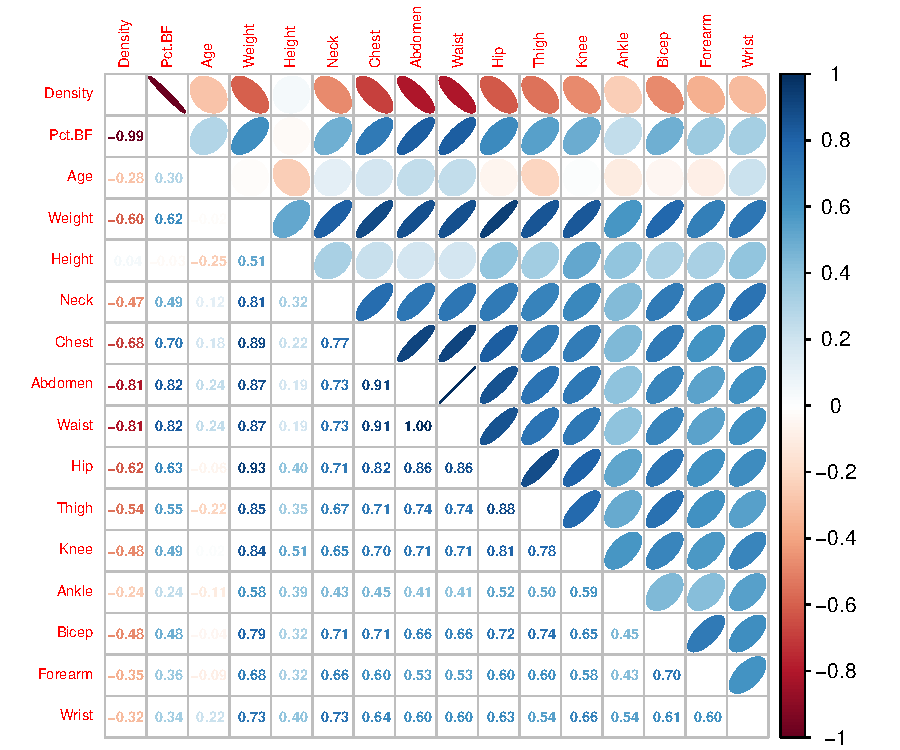
\includegraphics[width=0.66\textwidth, height=3.5in, page =1]{figure2}
  \end{center}
  \caption{Correlation Matrix Plot}\label{fig:corr}
\end{figure}

%\showmatmethods


\bibliography{pinp}
\bibliographystyle{jss}



\end{document}
